\documentclass{thesisreport}


\begin{document}

 \thispagestyle{empty}

\def\lskip{\vspace{0.5cm}}


\begin{tabular}{p{7cm}p{8cm}}
ÉCOLE CENTRALE DE NANTES
&
% EMARO students only
% \raggedleft FIRST YEAR INSTITUTION	
\end{tabular}

\vspace{2cm}

% CORO-IMARO students
\begin{center} \large\sc MASTER CORO-IMARO\\ \normalsize{``CONTROL and ROBOTICS''} \end{center}

% EMARO students
%\begin{center} \large\sc MASTER ERASMUS MUNDUS \\ \normalsize{EMARO+ ``European Master in Advanced Robotics''} \end{center}


\begin{center}
	2016 / 2017\\
	\lskip
	Master Thesis Report % or bibliography report
	\lskip
	
	Presented by \lskip 
	
	Student Name \lskip
	
	On Date \lskip\lskip
	
	{\Large \textbf{The title of the master thesis}}
	
	\vfill

Jury \lskip
		
	\end{center}
	


\begin{tabular}{p{3cm}p{7cm}p{5cm} }
 % President: & Name & Position (Institution) \\ & & \\     % for final defense only (not bibliography)
 Evaluators: & Name & Position (Institution) \\
	      & Name & Position (Institution) \\ 
	      & Name & Position (Institution) \\ & & \\  & & \\ 
  Supervisor(s):  & Name & Position (Institution) \\
		  & Name & Position (Institution) \\
% EMARO students only
%(EMARO)  & Co-supervisor from M1 & Position, M1 institution 
\end{tabular}

\lskip

\begin{flushleft}
 Laboratory: Laboratoire des Sciences du Numérique de Nantes LS2N
\end{flushleft}

\newpage
\thispagestyle{empty}
\null
\newpage
\addtocounter{page}{-1}
\pagestyle{fancy}
  
 
  \section*{Abstract}
   
 Do not forget to check each reference while importing in your Bibtex file.
 Especially, IEEExplore export may lead to ill-formatted conference name like \emph{Robotics and Automation, 
 IEEE International Conference on}.
 
 
 \newpage
 
 \section*{Acknowledgements}
 
 \newpage
 
 
 \section*{Notations}
 
 \newpage
 
  \section*{Abbreviations}
 
 \newpage
 
 \listoffigures
 
\listoftables
 
 \tableofcontents
 
 
 \chapter*{Introduction}
 \addcontentsline{toc}{chapter}{Introduction}	 % non-numbered chapters do not appear in table of contents by default
 
 
 \chapter{State of the art}
 
 \section{First topic}
 
 \section{Second topic}
 
 \chapter{Actual work}
  
 
 When dealing with rectangled triangles (see Figure \ref{triangle}) I sometimes used this theorem from \cite{pythm001}:
 \begin{equation}\label{theo}
  a^2 + b^2 = c^2
 \end{equation}The demonstration is in Appendix \ref{sec:prooftheorem}.
 
 \begin{figure}[h]\centering
  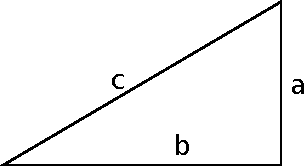
\includegraphics[width=.5\linewidth]{triangle1}
  \caption{A triangle with letters} \label{triangle}
 \end{figure}
 
 


 
 
 \chapter{Experiments}
 
 When trying to draw a rectangled triangle, my program comes up with Figure \ref{triangle2} that is neither rectangled nor a triangle.
 
  \begin{figure}[h]\centering
  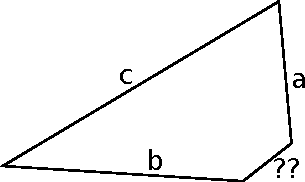
\includegraphics[width=.5\linewidth]{triangle2}
  \caption{Triangle drawn by my program. Note the 4th side.} \label{triangle2}
 \end{figure}
 
Unless there is a bug in my program, which is unlikely, this research indicates that the whole theory on triangles having 3 sides has been wrong for years, maybe decades.
 
 
 \chapter*{Conclusion}
 \addcontentsline{toc}{chapter}{Conclusion}
 
 
 
 
 
 % switch to A-B-C chaptering
 \appendix	
 
 \chapter{Proof of theorem \ref{theo}}
 \label{sec:prooftheorem}
 
 
 \begin{proof}
\eqref{theo} was already demonstrated in \cite{euclides300}.
\end{proof}
 
 \addcontentsline{toc}{chapter}{Bibliography}
 
 \bibliography{../biblio}
 
 
 
 
\end{document}
